\documentclass[conference]{IEEEtran}
\IEEEoverridecommandlockouts

\usepackage{cite}
\usepackage{amsmath,amssymb,amsfonts}
\usepackage{algorithmic}
\usepackage{graphicx}
\usepackage{textcomp}
\usepackage{booktabs}
\usepackage{tabularx}
\usepackage{adjustbox}
\usepackage{hyperref}
\usepackage{soul}
\usepackage[dvipsnames]{xcolor}
\usepackage{pifont}
\usepackage{array}

\def\BibTeX{{\rm B\kern-.05em{\sc i\kern-.025em b}\kern-.08em
    T\kern-.1667em\lower.7ex\hbox{E}\kern-.125emX}}

\begin{document}

\title{Implementation of DeFT: A Deadlock-Free and Fault-Tolerant Routing Algorithm for 2.5D Chiplet Networks}

\author{\IEEEauthorblockN{Yusuf Tahir Orhan - N24112049\IEEEauthorrefmark{1}}
\IEEEauthorblockA{\IEEEauthorrefmark{1}Computer Engineering Department,
Hacettepe University, Ankara, Turkey\\
\IEEEauthorrefmark{2}Graduate School of Science and Engineering,
Hacettepe University, Ankara, Turkey\\
E-mail: \IEEEauthorrefmark{1}yusuftahirorhan@hacettepe.edu.tr}
}

\maketitle

\begin{abstract}
This project implements and evaluates a Noxim-based \texttt{DEFT\_2\_5D} simulator extension for studying DeFT-style routing in a 2.5D chiplet network. The implementation models four chiplets on an active interposer, a deterministic physical Vertical Link (VL) inventory, startup permanent VL faults, DeFT virtual-network assignment rules, movement-transition filtering, schema-v1 offline VL lookup tables, explicit \texttt{XY} baseline modes, synthetic traffic profiles, machine-readable metrics export, and traceable experiment and analysis helpers. The final sweep completed 150 simulator runs across routing modes, traffic profiles, fault masks, and seeds. The generated results are valid for descriptive report support only. The measured data set contains empty and partial injection cells, including 54 completed runs with zero packets injected after the warm-up boundary. Therefore, this report presents finite-window measurements with coverage counts and limitations, while avoiding unsupported performance conclusions.
\end{abstract}

\begin{IEEEkeywords}
2.5D integration, chiplet networks, Network-on-Chip, deadlock-free routing, fault tolerance, Noxim.
\end{IEEEkeywords}

\section{Introduction}

2.5D chiplet integration connects multiple smaller dies through an active interposer. This architecture can improve modularity and yield, but it also makes inter-chiplet routing sensitive to VL availability and deadlock-avoidance constraints. DeFT is a routing approach proposed for this setting; it combines virtual-network assignment rules with fault-aware VL selection so inter-chiplet packets can be routed through the interposer while respecting deadlock-avoidance constraints~\cite{Taheri2022DeFT}.

The goal of this project is to extend the cycle-accurate Noxim simulator~\cite{Catania2016Noxim} so DeFT-style behavior can be studied in a reproducible workflow. The implementation focuses on a four-chiplet system with $4 \times 4$ chiplet-local meshes, a modeled active interposer layer, four physical bidirectional VLs per chiplet, permanent startup VL faults, two virtual channels for VN.0 and VN.1, and descriptive final metrics for reachability, average latency, and network throughput.

\textbf{Assumption:} The current implementation models 16 physical bidirectional VLs and uses the final-sweep policy recorded in the project documentation for reporting fault rates. This differs from single-direction endpoint fault modeling and is preserved as a limitation.

\begin{figure}[t]
    \centering
    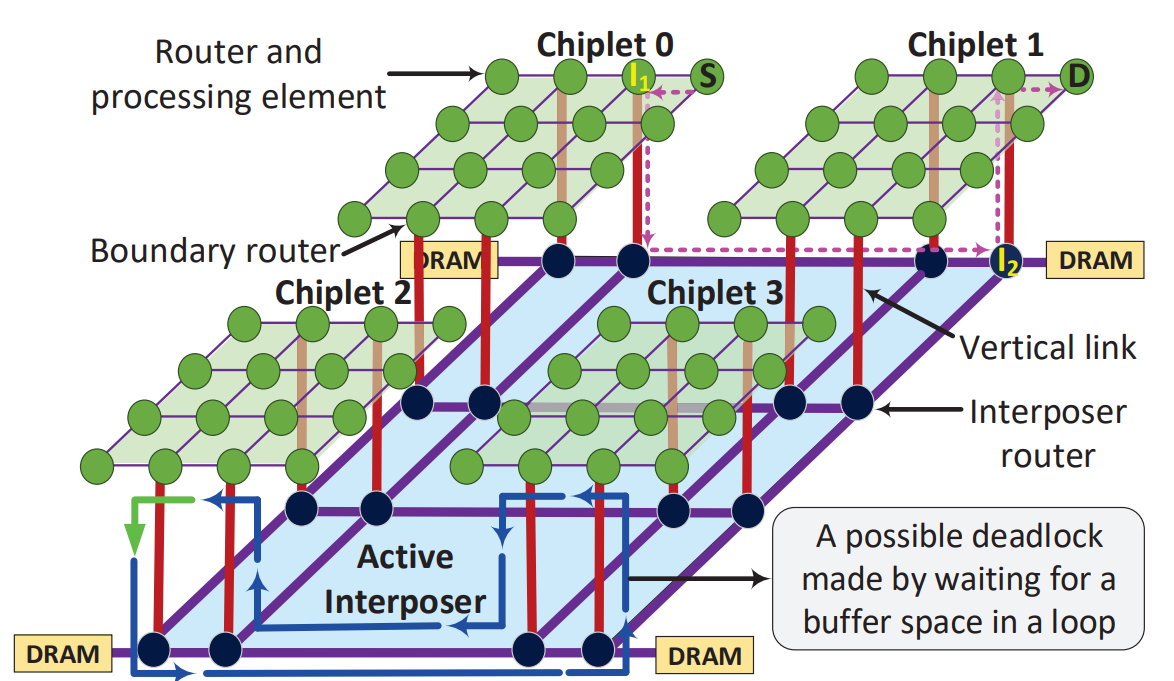
\includegraphics[width=\linewidth]{figures/schematic.png}
    \caption{Baseline 2.5D network architecture reused from the extended proposal source template.}
    \label{fig:architecture}
\end{figure}

\section{Related Work}

Routing for chiplet-based and interposer-based systems has been studied through several deadlock-avoidance and reliability mechanisms. Modular turn restriction approaches such as MTR restrict dependency cycles in chiplet systems~\cite{Yin2018MTR}. Remote-control and update-packet bypassing ideas explore alternate mechanisms for modular systems and 2.5D deadlock handling~\cite{Majumder2020RC,Wang2023BUP}. ReD extends the virtual-network reliability direction for 2.5D interposer systems~\cite{Taheri2023ReD}. Fault-tolerant 3D NoC routing and configurable inter-die links provide related reliability context, but their assumptions differ from the up-down-up communication pattern of active-interposer 2.5D systems~\cite{Salamat2018Runtime,Li2020Circular,Hsu2015Link}.

This project uses the original DeFT paper as the primary algorithmic reference for virtual-network assignment, movement restrictions, and design-time VL selection~\cite{Taheri2022DeFT}. The implementation does not claim a new formal proof; it implements and validates the documented project surfaces inside Noxim.

\section{Problem Definition}

The project problem is to support deadlock-free and fault-tolerant inter-chiplet routing in a modeled 2.5D system while preserving traceable simulator behavior. The target topology contains four CPU chiplets integrated on an active interposer. Each chiplet contains a $4 \times 4$ mesh, and each chiplet has four physical bidirectional VLs located at boundary routers.

The evaluation target from the project requirements is synthetic traffic under permanent VL fault scenarios, using reachability, latency, and throughput metrics. The implemented synthetic profiles are uniform, localized with 40\% same-chiplet traffic probability, and hotspot traffic with three deterministic hotspot routers. Real-application PARSEC/GEM5 trace evaluation remains outside the current validated artifact set; PARSEC is a benchmark suite reference point, but no PARSEC/GEM5 trace workflow is validated in this final report~\cite{Bienia2011PARSEC}.

\textbf{Blocked:} Real-application PARSEC/GEM5 trace evaluation would require a separate documented setup and validation task before inclusion.

\section{System Architecture and Design}

\subsection{Topology Model}

The \texttt{DEFT\_2\_5D} topology uses a $2 \times 2$ chiplet grid. Chiplet router IDs are \texttt{0..63}; interposer router IDs are \texttt{64..127}. Packet sources and final destinations remain chiplet routers only. The interposer routers are internal transit routers.

Each chiplet owns four physical bidirectional VLs at deterministic boundary routers. The current model therefore has 16 physical bidirectional VLs. These physical links can also be described as 32 directional-equivalent channels for paper-aligned fault-rate reporting, but the simulator fault model disables one physical bidirectional VL as one object.

\subsection{Virtual Networks}

For \texttt{DEFT\_2\_5D}, VN.0 maps to VC 0 and VN.1 maps to VC 1. This avoids a parallel virtual-network field and keeps the routing state aligned with the existing Noxim virtual-channel flow-control path. Boundary-router reassignment is output-VC-aware so a head flit can reserve and forward into the selected VN safely.

The implemented movement filter enforces the current VN transition restrictions: VN.1 to VN.0 is rejected, Up-to-Horizontal movement in VN.0 is rejected, and Horizontal-to-Down movement in VN.1 is rejected. Because explicit Up and Down ports do not exist in the original Noxim direction set, the current implementation derives movement context from the layer, boundary-router state, input direction, and output direction.

\subsection{VL Lookup Tables}

The offline LUT generator emits a versioned \texttt{deft\_vl\_lut.v1} YAML format. Runtime DeFT routing loads the schema-v1 LUT, derives the active physical fault mask from current VL state, and selects source-side exit and destination-side entry VL records by lookup. Missing entries or nonfunctional selected VLs fail closed by returning no legal output direction.

\section{Implementation}

The project was implemented task by task and recorded in \path{docs/TASKS.md}, \path{docs/PROGRESS.md}, \path{docs/ARCHITECTURE.md}, and \path{docs/DECISIONS.md}. Main implemented surfaces are:

\begin{itemize}
    \item \path{external/noxim/src/DeftTopology.*}: layer-aware router mapping, physical VL records, boundary-router inventory, and topology validation.
    \item \path{external/noxim/src/DeftFaultInjectionManager.*}: startup permanent physical VL fault configuration and validation.
    \item \path{external/noxim/src/DeftVirtualNetwork.*}: VN/VC mapping helpers and DeFT VN assignment support.
    \item \path{external/noxim/src/routingAlgorithms/Routing_DEFT.*}: runtime DeFT route selection through schema-v1 VL LUT entries.
    \item \path{external/noxim/src/DeftVerticalLinkLut.*}: schema-v1 VL LUT loader and validator.
    \item \path{external/noxim/config_examples/}: \texttt{DEFT\_2\_5D} topology, \texttt{XY} baselines, and synthetic traffic configurations.
    \item \path{external/noxim/other/deft_vl_lut_generator.py}: deterministic offline VL LUT generator.
    \item \path{external/noxim/other/deft_experiment_runner.py}: traceable experiment launcher.
    \item \path{external/noxim/other/deft_analysis_artifacts.py}: mechanical final-analysis artifact generator.
    \item \path{external/noxim/src/GlobalStats.*} and \path{external/noxim/src/ProcessingElement.*}: machine-readable metrics export and injected-packet counters.
\end{itemize}

\textbf{Assumption:} Generated artifacts under \path{external/noxim/other/generated/} are report-support outputs and remain traceable to their manifests.

\section{Experimental Setup}

The final sweep policy was defined before running the final matrix and was executed without changing simulator behavior during report drafting. Table~\ref{tab:setup} summarizes the matrix. The final sweep contains exactly 150 planned and completed simulator runs. No post-injection drain phase is included in the current fixed-window policy.

\begin{table}[t]
\centering
\caption{Final Sweep Matrix}
\label{tab:setup}
\begin{tabularx}{\columnwidth}{@{}lX@{}}
\toprule
\textbf{Dimension} & \textbf{Values} \\
\midrule
Routing modes & \texttt{XY}, \texttt{DEFT} \\
Traffic profiles & \texttt{uniform}, \texttt{localized\_40}, \texttt{hotspot\_3x10} \\
Fault masks & \texttt{0x0000}, \texttt{0x0001}, \texttt{0x0011}, \texttt{0x0111}, \texttt{0x1111} \\
Physical fault rates & 0\%, 6.25\%, 12.5\%, 18.75\%, 25\% \\
Seeds & \texttt{0}, \texttt{1}, \texttt{2}, \texttt{3}, \texttt{4} \\
Simulation window & \texttt{-sim 10000} \\
Warm-up window & \texttt{-warmup 1000} \\
Stats format & JSON \\
\bottomrule
\end{tabularx}
\end{table}

\textbf{Assumption:} A zero-injection run is a completed simulator run with \texttt{total\_injected\_packets == 0} in the measured stats window, not a failed run.

\textbf{Blocked:} The current runner policy does not evaluate eventual delivery after a post-injection drain phase.

\textbf{Blocked:} The current physical bidirectional fault model does not represent the original paper's single-direction 3.125\% fault case.

\section{Validation Provenance}

The final report-support results are traceable through the following generated artifacts:

\begin{itemize}
    \item T0026 final sweep output: \path{external/noxim/other/generated/t0026_final_sweep_v1/}.
    \item T0026 final analysis output: \path{external/noxim/other/generated/t0026_final_analysis_v1/}.
    \item T0027 report-support output: \path{external/noxim/other/generated/t0027_report_support_v1/}.
    \item T0028 claim-safe results draft: \path{external/noxim/other/generated/t0028_final_report_results_v1/report_results_draft.md}.
\end{itemize}

T0026 validation established that the executed manifest had \texttt{mode: execute}, \texttt{run\_count: 150}, 150 completed runs, and 150 return code 0 runs. All 150 JSON stats files existed and contained the T0020 metric fields. T0027 validation derived blank-aware condition and pair tables from T0026 raw artifacts and cross-checked them against the T0026 sweep summary, analysis run summary, and analysis comparison summary. T0028 converted the T0027 report-support tables into claim-safe prose and Markdown tables without rerunning simulations. The T0028 manifest keeps \texttt{claims\_allowed: false}.

\section{Results and Evaluation}

The results in this section are assembled from the reviewed Markdown draft and the T0028/T0027/T0026 report-support artifacts. They are finite-window descriptive measurements. Blank cells are intentional and indicate that the supporting denominator is absent.

All 150 planned simulator runs completed with return code 0, and the generated T0027 report-support tables were cross-checked against the T0026 executed manifest, raw JSON stats, sweep summary, analysis run summary, and analysis comparison summary with zero mismatches. The upstream report-support manifest keeps \texttt{claims\_allowed: false}.

The measured data set contains completed runs in which no packets were injected after the warm-up boundary. T0027 records 54 individual zero-injection runs. At condition level, 12 cells have packet injection in all five seeds, 13 cells have packet injection in only some seeds, and 5 cells have no packet injection in any seed. The 5 empty-injection cells are all \texttt{XY} with \texttt{hotspot\_3x10} traffic.

Under this fixed-window measurement policy, the \texttt{XY} hotspot cells cannot be compared with \texttt{DEFT} because the \texttt{XY} side injected zero packets in every hotspot fault-mask cell. The \texttt{XY} uniform and localized cells injected packets in some seeds, but received zero packets in the measured window. Therefore, side-by-side latency comparisons against \texttt{DEFT} are not supported.

\subsection{Artifact Readiness}

\begin{table}[t]
\centering
\caption{Artifact and Readiness Summary}
\label{tab:readiness}
\begin{tabular}{@{}lr@{}}
\toprule
\textbf{Item} & \textbf{Value} \\
\midrule
Planned and completed runs & 150 \\
Raw stats rows & 150 \\
Condition cells & 30 \\
XY/DEFT pair rows & 15 \\
Individual zero-injection runs & 54 \\
Complete-injection condition cells & 12 \\
Partial-injection condition cells & 13 \\
Empty-injection condition cells & 5 \\
Cross-check mismatches & 0 \\
Claim state & \texttt{claims\_allowed: false} \\
\bottomrule
\end{tabular}
\end{table}

\subsection{Coverage}

\begin{table}[t]
\centering
\caption{Coverage by Routing and Traffic}
\label{tab:coverage}
\begin{adjustbox}{max width=\columnwidth}
\begin{tabular}{@{}llrrrrr@{}}
\toprule
\textbf{Routing} & \textbf{Traffic} & \textbf{Runs} & \textbf{Nonempty} & \textbf{Zero} & \textbf{Injected} & \textbf{Received} \\
\midrule
\texttt{DEFT} & \texttt{hotspot\_3x10} & 25 & 22 & 3 & 336 & 134 \\
\texttt{DEFT} & \texttt{localized\_40} & 25 & 25 & 0 & 1016 & 542 \\
\texttt{DEFT} & \texttt{uniform} & 25 & 24 & 1 & 436 & 238 \\
\texttt{XY} & \texttt{hotspot\_3x10} & 25 & 0 & 25 & 0 & 0 \\
\texttt{XY} & \texttt{localized\_40} & 25 & 20 & 5 & 35 & 0 \\
\texttt{XY} & \texttt{uniform} & 25 & 5 & 20 & 5 & 0 \\
\bottomrule
\end{tabular}
\end{adjustbox}
\end{table}

\subsection{Condition-Level Metrics}

Reachability is \texttt{total\_received\_packets / total\_injected\_packets} within the condition. Latency is received-packet-weighted across runs with received packets. Mean network throughput is the exported finite-window mean across all five runs. Status codes are: C = \texttt{complete\_injection\_cell}, P = \texttt{partial\_injection\_cell}, and E = \texttt{empty\_injection\_cell}. Blank reachability means no injected-packet denominator exists. Blank latency means no received-packet delay samples exist.

\begin{table*}[t]
\centering
\caption{Condition-Level Descriptive Metrics}
\label{tab:condition_metrics}
\scriptsize
\setlength{\tabcolsep}{3pt}
\begin{adjustbox}{max width=\textwidth}
\begin{tabular}{@{}lllrrrrrrrrl@{}}
\toprule
\textbf{Routing} & \textbf{Traffic} & \textbf{Mask} & \textbf{Fault} & \textbf{Nonempty} & \textbf{Empty} & \textbf{Inj.} & \textbf{Recv.} & \textbf{Reach.} & \textbf{Latency} & \textbf{Thput.} & \textbf{Status} \\
\midrule
\texttt{DEFT} & \texttt{hotspot\_3x10} & \texttt{0x0000} & 0 & 5 & 0 & 69 & 19 & 0.27536232 & 12.73684211 & 0.0034222222 & C \\
\texttt{DEFT} & \texttt{hotspot\_3x10} & \texttt{0x0001} & 6.25 & 4 & 1 & 19 & 4 & 0.21052632 & 16.75 & 0.0007111111 & P \\
\texttt{DEFT} & \texttt{hotspot\_3x10} & \texttt{0x0011} & 12.5 & 3 & 2 & 114 & 72 & 0.63157895 & 40.36111111 & 0.0126888889 & P \\
\texttt{DEFT} & \texttt{hotspot\_3x10} & \texttt{0x0111} & 18.75 & 5 & 0 & 66 & 18 & 0.27272727 & 7.61111111 & 0.0034666667 & C \\
\texttt{DEFT} & \texttt{hotspot\_3x10} & \texttt{0x1111} & 25 & 5 & 0 & 68 & 21 & 0.30882353 & 9.47619048 & 0.0043333333 & C \\
\texttt{DEFT} & \texttt{localized\_40} & \texttt{0x0000} & 0 & 5 & 0 & 289 & 166 & 0.57439446 & 23.37951807 & 0.0294888889 & C \\
\texttt{DEFT} & \texttt{localized\_40} & \texttt{0x0001} & 6.25 & 5 & 0 & 144 & 72 & 0.5 & 16.83333333 & 0.0129777778 & C \\
\texttt{DEFT} & \texttt{localized\_40} & \texttt{0x0011} & 12.5 & 5 & 0 & 114 & 60 & 0.52631579 & 16.08333333 & 0.0112 & C \\
\texttt{DEFT} & \texttt{localized\_40} & \texttt{0x0111} & 18.75 & 5 & 0 & 303 & 155 & 0.51155116 & 18.50967742 & 0.0285111111 & C \\
\texttt{DEFT} & \texttt{localized\_40} & \texttt{0x1111} & 25 & 5 & 0 & 166 & 89 & 0.53614458 & 18.43820225 & 0.0160888889 & C \\
\texttt{DEFT} & \texttt{uniform} & \texttt{0x0000} & 0 & 5 & 0 & 82 & 38 & 0.46341463 & 24.23684211 & 0.0071555556 & C \\
\texttt{DEFT} & \texttt{uniform} & \texttt{0x0001} & 6.25 & 5 & 0 & 137 & 84 & 0.61313869 & 23.96428571 & 0.0149777778 & C \\
\texttt{DEFT} & \texttt{uniform} & \texttt{0x0011} & 12.5 & 5 & 0 & 63 & 17 & 0.26984127 & 22.23529412 & 0.0032888889 & C \\
\texttt{DEFT} & \texttt{uniform} & \texttt{0x0111} & 18.75 & 5 & 0 & 81 & 49 & 0.60493827 & 20.08163265 & 0.0086 & C \\
\texttt{DEFT} & \texttt{uniform} & \texttt{0x1111} & 25 & 4 & 1 & 73 & 50 & 0.68493151 & 21.9 & 0.0087555556 & P \\
\texttt{XY} & \texttt{hotspot\_3x10} & \texttt{0x0000} & 0 & 0 & 5 & 0 & 0 & & & 0 & E \\
\texttt{XY} & \texttt{hotspot\_3x10} & \texttt{0x0001} & 6.25 & 0 & 5 & 0 & 0 & & & 0 & E \\
\texttt{XY} & \texttt{hotspot\_3x10} & \texttt{0x0011} & 12.5 & 0 & 5 & 0 & 0 & & & 0 & E \\
\texttt{XY} & \texttt{hotspot\_3x10} & \texttt{0x0111} & 18.75 & 0 & 5 & 0 & 0 & & & 0 & E \\
\texttt{XY} & \texttt{hotspot\_3x10} & \texttt{0x1111} & 25 & 0 & 5 & 0 & 0 & & & 0 & E \\
\texttt{XY} & \texttt{localized\_40} & \texttt{0x0000} & 0 & 4 & 1 & 7 & 0 & 0 & & 0 & P \\
\texttt{XY} & \texttt{localized\_40} & \texttt{0x0001} & 6.25 & 4 & 1 & 7 & 0 & 0 & & 0 & P \\
\texttt{XY} & \texttt{localized\_40} & \texttt{0x0011} & 12.5 & 4 & 1 & 7 & 0 & 0 & & 0 & P \\
\texttt{XY} & \texttt{localized\_40} & \texttt{0x0111} & 18.75 & 4 & 1 & 7 & 0 & 0 & & 0 & P \\
\texttt{XY} & \texttt{localized\_40} & \texttt{0x1111} & 25 & 4 & 1 & 7 & 0 & 0 & & 0 & P \\
\texttt{XY} & \texttt{uniform} & \texttt{0x0000} & 0 & 1 & 4 & 1 & 0 & 0 & & 0 & P \\
\texttt{XY} & \texttt{uniform} & \texttt{0x0001} & 6.25 & 1 & 4 & 1 & 0 & 0 & & 0 & P \\
\texttt{XY} & \texttt{uniform} & \texttt{0x0011} & 12.5 & 1 & 4 & 1 & 0 & 0 & & 0 & P \\
\texttt{XY} & \texttt{uniform} & \texttt{0x0111} & 18.75 & 1 & 4 & 1 & 0 & 0 & & 0 & P \\
\texttt{XY} & \texttt{uniform} & \texttt{0x1111} & 25 & 1 & 4 & 1 & 0 & 0 & & 0 & P \\
\bottomrule
\end{tabular}
\end{adjustbox}
\end{table*}

\subsection{Pairwise Readiness}

No delta columns are included. Table~\ref{tab:pair_readiness} describes whether values can be displayed side by side, not whether either routing mode should be preferred. The readiness code \texttt{XY-empty} means the XY side injected zero packets in the measured cell. The readiness code \texttt{latency-blank} means both modes have injection, but one mode has zero received packets, so latency comparison is blank.

\begin{table*}[t]
\centering
\caption{XY/DEFT Pairwise Readiness}
\label{tab:pair_readiness}
\scriptsize
\begin{adjustbox}{max width=\textwidth}
\begin{tabular}{@{}lllll@{}}
\toprule
\textbf{Traffic} & \textbf{Fault mask} & \textbf{XY status} & \textbf{DEFT status} & \textbf{Readiness} \\
\midrule
\texttt{hotspot\_3x10} & \texttt{0x0000} & E & C & \texttt{XY-empty} \\
\texttt{hotspot\_3x10} & \texttt{0x0001} & E & P & \texttt{XY-empty} \\
\texttt{hotspot\_3x10} & \texttt{0x0011} & E & P & \texttt{XY-empty} \\
\texttt{hotspot\_3x10} & \texttt{0x0111} & E & C & \texttt{XY-empty} \\
\texttt{hotspot\_3x10} & \texttt{0x1111} & E & C & \texttt{XY-empty} \\
\texttt{localized\_40} & \texttt{0x0000} & P & C & \texttt{latency-blank} \\
\texttt{localized\_40} & \texttt{0x0001} & P & C & \texttt{latency-blank} \\
\texttt{localized\_40} & \texttt{0x0011} & P & C & \texttt{latency-blank} \\
\texttt{localized\_40} & \texttt{0x0111} & P & C & \texttt{latency-blank} \\
\texttt{localized\_40} & \texttt{0x1111} & P & C & \texttt{latency-blank} \\
\texttt{uniform} & \texttt{0x0000} & P & C & \texttt{latency-blank} \\
\texttt{uniform} & \texttt{0x0001} & P & C & \texttt{latency-blank} \\
\texttt{uniform} & \texttt{0x0011} & P & C & \texttt{latency-blank} \\
\texttt{uniform} & \texttt{0x0111} & P & C & \texttt{latency-blank} \\
\texttt{uniform} & \texttt{0x1111} & P & P & \texttt{latency-blank} \\
\bottomrule
\end{tabular}
\end{adjustbox}
\end{table*}

\subsection{Zero-Injection Runs}

The full 54-run list is preserved in \path{external/noxim/other/generated/t0027_report_support_v1/zero_injection_runs.csv}. Table~\ref{tab:zero_injection} summarizes the zero-injection rows by routing and traffic profile.

\begin{table}[t]
\centering
\caption{Zero-Injection Run Summary}
\label{tab:zero_injection}
\begin{tabular}{@{}llr@{}}
\toprule
\textbf{Routing} & \textbf{Traffic} & \textbf{Zero-injection runs} \\
\midrule
\texttt{DEFT} & \texttt{hotspot\_3x10} & 3 \\
\texttt{DEFT} & \texttt{uniform} & 1 \\
\texttt{XY} & \texttt{hotspot\_3x10} & 25 \\
\texttt{XY} & \texttt{localized\_40} & 5 \\
\texttt{XY} & \texttt{uniform} & 20 \\
\bottomrule
\end{tabular}
\end{table}

\section{Limitations}

\textbf{Assumption:} The final report text is descriptive support, not a new analysis layer.

\textbf{Assumption:} Aggregated reachability is blank when no packets were injected.

\textbf{Assumption:} Latency is blank when no packets were received.

\textbf{Blocked:} Empty or partial injection cells cannot support unqualified performance claims.

\textbf{Blocked:} \texttt{XY} hotspot cells injected zero packets for all seeds and fault masks in the measured window.

\textbf{Blocked:} The current data set does not support \texttt{XY}/\texttt{DEFT} latency comparisons because the \texttt{XY} side has zero received packets wherever it injected packets.

\textbf{Blocked:} Stronger result statements, non-empty \texttt{XY} hotspot measurements, latency comparisons, single-direction fault cases, and eventual-delivery checks require separate documented validation or rerun policy.

\textbf{Blocked:} PARSEC/GEM5 trace evaluation remains outside the current final-sweep artifact set.

\section{Reproducibility}

The final LaTeX artifact is generated from \path{docs/FINAL_REPORT_DRAFT.md}, using \path{Extended_Proposal.zip} as the IEEE conference-style template reference. The final report source is intentionally separated from the extended proposal source so the original archive and proposal files remain unchanged.

The report-support data are traceable through task IDs T0025 through T0028. The simulator final sweep was not rerun during final-report conversion. The report conversion task creates only LaTeX artifact files and tracking-document updates.

\section{Conclusion and Future Work}

The project produced a traceable Noxim extension for \texttt{DEFT\_2\_5D} and a reproducible final-sweep artifact set. The final report-support data confirms that the planned 150-run matrix executed successfully and that generated summary tables cross-check against raw artifacts. The reportable results should remain descriptive because the measured fixed-window data contains blank and partial cells.

The safest conclusion is that the implementation and report-support workflow are in place, while stronger experimental claims require an explicitly scoped follow-up validation policy. Future work should address non-empty hotspot measurements for the \texttt{XY} baseline, a post-injection drain policy for eventual-delivery checks, directional endpoint fault modeling, traffic-profile-specific LUT demand inputs, and validated PARSEC/GEM5 trace support before expanding the report claims.

\bibliographystyle{IEEEtran}
\bibliography{references}

\end{document}
